\section{Results}
\label{sec:results}

\subsection{Overall Probe Accuracy}

\Tabref{tab:main_results} presents the main results. All four formats encode recoverable base-10 digit information, with word-form formats achieving substantially higher accuracy than digit strings.

\begin{table}[t]
    \centering
    \caption{Overall probe accuracy at each format's best layer. We report accuracy (all three digits correct) with 95\% confidence intervals from the single best seed, and mean $\pm$ std across 5 random seeds. Word-form representations significantly outperform digit string representations. Best single-seed result in \textbf{bold}.}
    \begin{tabular}{@{}lcccr@{}}
        \toprule
        \textbf{Format} & \textbf{Best Layer} & \textbf{Accuracy (\%)} & \textbf{95\% CI} & \textbf{5-seed Mean} \\
        \midrule
        \digits       & 31 & 91.0 & [87.0, 94.5] & 85.5 {\scriptsize $\pm$ 1.6} \\
        \english      & 8  & 98.5 & [96.5, 100]  & 97.0 {\scriptsize $\pm$ 1.0} \\
        \francefr     & 6  & 98.0 & [96.0, 99.5] & 95.2 {\scriptsize $\pm$ 1.9} \\
        \belgianfr    & 6  & \textbf{99.0} & [97.5, 100]  & 97.7 {\scriptsize $\pm$ 0.7} \\
        \bottomrule
    \end{tabular}
    \label{tab:main_results}
\end{table}

\francefr achieves 98.0\% accuracy despite the vigesimal arithmetic structure of numbers 70--99. This is comparable to \english (98.5\%) and only 1 percentage point below \belgianfr (99.0\%). The difference between \francefr and \english is not statistically significant (McNemar's $\chi^2 = 0.00$, $p = 1.000$), nor is the difference between \francefr and \belgianfr ($\chi^2 = 0.25$, $p = 0.617$). However, \francefr significantly outperforms \digits ($\chi^2 = 9.39$, $p = 0.002$): of the 18 digit-string errors, 16 were correctly predicted by the French probe.

Across 5 random seeds, \francefr averages 95.2\% $\pm$ 1.9\%, confirming the robustness of the finding. \belgianfr is the most stable format (97.7\% $\pm$ 0.7\%).

\subsection{Vigesimal vs.\ Decimal Accuracy}

\Tabref{tab:vigesimal} breaks down \francefr accuracy by number range. The vigesimal range (70--99) shows slightly lower accuracy (96.7\%) than the decimal range (98.6\%), but this difference is not statistically significant (Fisher's exact test, $p = 0.585$).

\begin{table}[t]
    \centering
    \caption{Probe accuracy for \francefr stratified by number range. The \emph{soixante-dix} (70--79) range shows the lowest accuracy, while \emph{quatre-vingts} (80--89) and \emph{quatre-vingt-dix} (90--99) achieve perfect accuracy. Best result in \textbf{bold}.}
    \begin{tabular}{@{}lccc@{}}
        \toprule
        \textbf{Range} & \textbf{$n$} & \textbf{Accuracy (\%)} & \textbf{Structure} \\
        \midrule
        All numbers         & 200 & 98.0 & --- \\
        \midrule
        Decimal (0--69)     & 140 & 98.6 & Standard \\
        Vigesimal (70--99)  & 60  & 96.7 & Base-20 \\
        \midrule
        \quad 70--79 (\emph{soixante-dix})    & 17  & 88.2 & $60+10+x$ \\
        \quad 80--89 (\emph{quatre-vingts})   & 22  & \textbf{100}  & $4\times20+x$ \\
        \quad 90--99 (\emph{quatre-vingt-dix}) & 21 & \textbf{100}  & $4\times20+10+x$ \\
        \bottomrule
    \end{tabular}
    \label{tab:vigesimal}
\end{table}

The breakdown by vigesimal sub-range is revealing. The \emph{soixante-dix} (70--79) range drops to 88.2\% accuracy, while the \emph{quatre-vingts} (80--89) and \emph{quatre-vingt-dix} (90--99) ranges achieve perfect 100\% accuracy. This asymmetry is striking: the 80s and 90s use ``quatre-vingt'' ($4\times20$) as a stem, which the model handles perfectly, but the 70s use ``soixante'' (60) plus a teens number, which introduces ambiguity.

In contrast, \belgianfr achieves 100\% accuracy on all three vigesimal sub-ranges, confirming that the decimal naming system (\emph{septante}, \emph{huitante}, \emph{nonante}) produces uniformly clean representations.

\subsection{Layer-wise Analysis}
\label{sec:layer_analysis}

\Figref{fig:layer_analysis} shows probe accuracy as a function of transformer layer. The most striking finding is the divergence in peak layers between word-form and digit-string formats.

\begin{figure}[t]
    \centering
    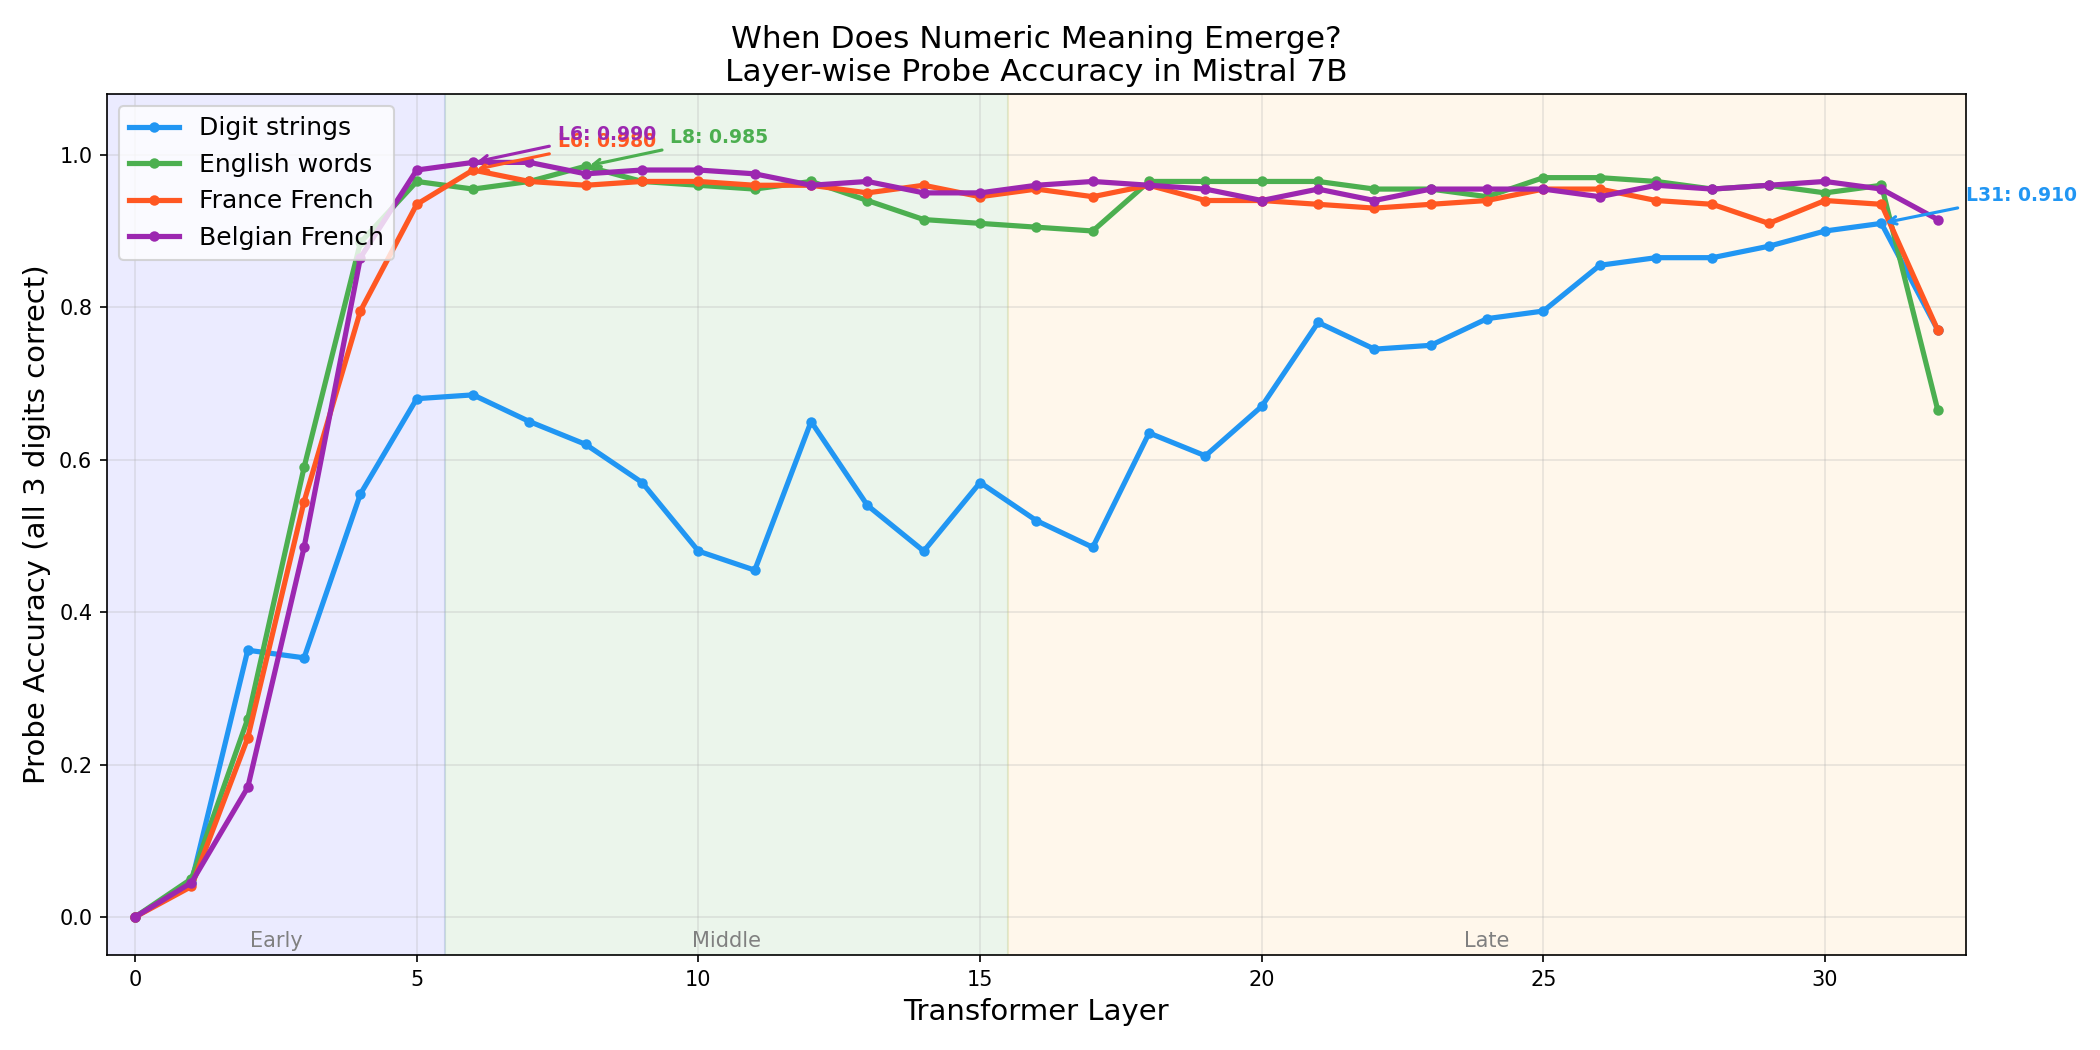
\includegraphics[width=0.95\linewidth]{figures/layer_peak_analysis.png}
    \caption{Probe accuracy across transformer layers for all four input formats. Word-form representations (\english, \francefr, \belgianfr) peak at early layers (5--8), while \digits peaks at the final layer (31). All three word-form formats first exceed 90\% accuracy at layer 5.}
    \label{fig:layer_analysis}
\end{figure}

All three word-form formats (\english, \francefr, \belgianfr) first exceed 90\% accuracy at layer 5 and peak between layers 6 and 8. \digits, by contrast, does not reach 90\% until layer 31 and peaks at layer 31. This means the model extracts numeric meaning from word-form numbers within the first 15--20\% of its depth, while digit-string representations require essentially the full network.

\Tabref{tab:layer_emergence} summarizes the layer dynamics.

\begin{table}[t]
    \centering
    \caption{Layer at which probe accuracy first exceeds 90\% and the peak accuracy layer for each format. Word-form numbers achieve high accuracy much earlier in the network than digit strings.}
    \begin{tabular}{@{}lcc@{}}
        \toprule
        \textbf{Format} & \textbf{First Layer $\geq$90\%} & \textbf{Peak Layer} \\
        \midrule
        \digits       & 31 & 31 \\
        \english      & 5  & 8  \\
        \francefr     & 5  & 6  \\
        \belgianfr    & 5  & 6  \\
        \bottomrule
    \end{tabular}
    \label{tab:layer_emergence}
\end{table}

\subsection{Error Analysis}
\label{sec:errors}

\Tabref{tab:errors_french} lists all four \francefr errors. Two errors (73, 76) show a clear pattern: the probe decodes the ``soixante'' (60) component literally, predicting a tens digit of 6 instead of 7.

\begin{table}[t]
    \centering
    \caption{All \francefr errors on the test set. The soixante-dix errors reveal partial arithmetic decomposition: the probe recovers ``soixante'' as 6 in the tens digit rather than the composed value 7.}
    \begin{tabular}{@{}cclll@{}}
        \toprule
        \textbf{True} & \textbf{Predicted} & \textbf{French Word} & \textbf{Error Type} & \textbf{Pattern} \\
        \midrule
        0   & 4   & z\'ero               & Units: $0 \to 4$  & Edge case \\
        73  & 63  & soixante-treize      & Tens: $7 \to 6$   & soixante $= 60$ \\
        76  & 66  & soixante-seize       & Tens: $7 \to 6$   & soixante $= 60$ \\
        116 & 106 & cent-seize           & Tens: $1 \to 0$   & Teen confusion \\
        \bottomrule
    \end{tabular}
    \label{tab:errors_french}
\end{table}

The soixante-dix errors are particularly informative. For 73 (``soixante-treize,'' literally ``sixty-thirteen''), the probe predicts 63---recovering ``soixante'' as 60 and ``treize'' as 3, but failing to compose $60+13=73$. The same pattern appears for 76 (``soixante-seize'' $\to$ 66 instead of 76). This suggests that the model's representation partially reflects the compositional arithmetic structure rather than the final composed value.

The ``quatre-vingts'' (80s) and ``quatre-vingt-dix'' (90s) ranges show no errors. This may be because ``quatre-vingt'' functions as a more unitized lexical stem: it always maps to 8 in the tens digit (for 80--89) or 9 (for 90--99 via ``quatre-vingt-dix''), whereas ``soixante'' can map to either 6 (for 60--69) or 7 (for 70--79), creating genuine ambiguity.

By comparison, the 18 \digits errors are scattered across the number range without clear arithmetic patterns, likely reflecting tokenization artifacts rather than systematic arithmetic confusion.
